\renewcommand*{\arraystretch}{1.1}

\noindent\begin{tabularx}{17cm}{|p{1.95cm}|X|}
	\hline
	number      & 4                                                          \\ \hline
%
	title       & Popular topics in a country                                                           \\ \hline
	\multicolumn{2}{|c|}{ 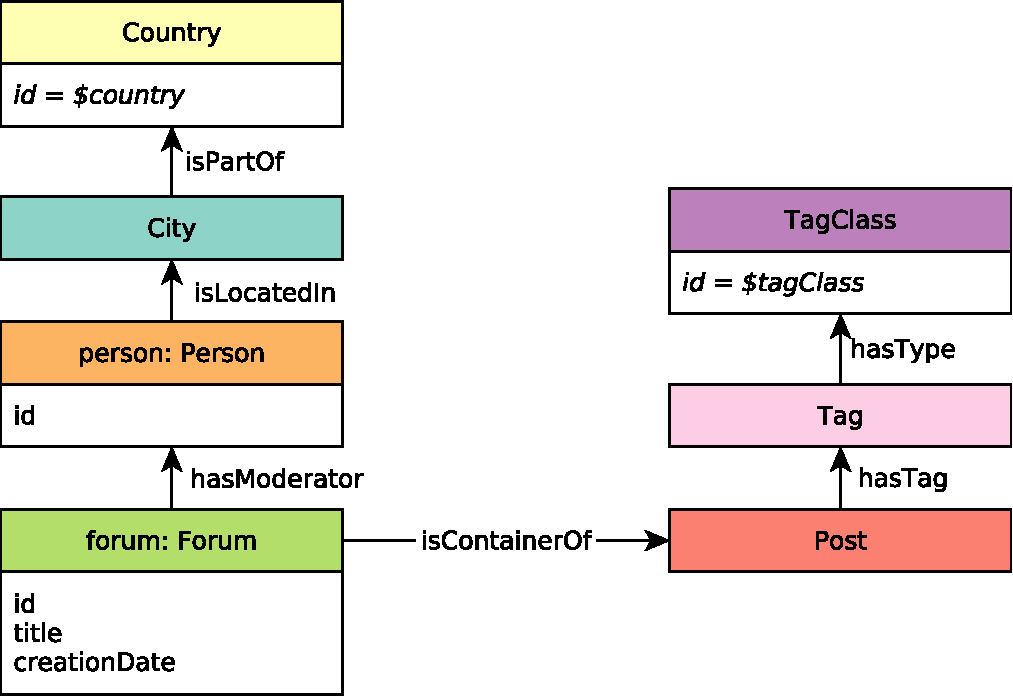
\includegraphics[scale=\patternscale,margin=0cm .2cm]{patterns/q04}} \\ \hline
	description & Given a TagClass and a Country, find all the Forums created in the given
Country, containing at least one Post with Tags belonging directly to
the given TagClass.

The location of a Forum is identified by the location of the Forum's
moderator.

TODO - what do we count, Posts? (szarnyasg)
 \\ \hline
	
%
	parameters  &
	\vspace{1.1ex}{\begin{tabularx}{14.38cm}{|c|M|m{2cm}|Y} \hline
	\cellcolor{black!70} \color{white} $\mathsf{1}$ & \varname{tagClass} & \cellcolor{gray!20} \vartype{32-bit Integer} &  \\\hline
	\cellcolor{black!70} \color{white} $\mathsf{2}$ & \varname{country} & \cellcolor{gray!20} \vartype{32-bit Integer} &  \\
	\end{tabularx}} \\ \hline
%
	result      &
	\vspace{1.1ex}{\begin{tabularx}{14.38cm}{|c|M|m{2cm}|Y} \hline
	\cellcolor{black!70} \color{white} $\mathsf{1}$ & \varname{forum.id} & \cellcolor{gray!20} \vartype{64-bit Integer} &  \\\hline
	\cellcolor{black!70} \color{white} $\mathsf{2}$ & \varname{forum.title} & \cellcolor{gray!20} \vartype{String} &  \\\hline
	\cellcolor{black!70} \color{white} $\mathsf{3}$ & \varname{forum.creationDate} & \cellcolor{gray!20} \vartype{DateTime} &  \\\hline
	\cellcolor{black!70} \color{white} $\mathsf{4}$ & \varname{person.id} & \cellcolor{gray!20} \vartype{64-bit Integer} &  \\\hline
	\cellcolor{black!70} \color{white} $\mathsf{5}$ & \varname{count} & \cellcolor{gray!20} \vartype{32-bit Integer} &  \\
	\end{tabularx}} \\ \hline
	%
	sort        &
	\vspace{1.1ex}{\begin{tabular}{|c|l|c|} \hline
	\cellcolor{black!70} \color{white} $\mathsf{1}$ & \varname{count} & \cellcolor{gray!20} $\desc$ \\\hline
	\cellcolor{black!70} \color{white} $\mathsf{2}$ & \varname{forum.id} & \cellcolor{gray!20} $\asc$ \\
	\end{tabular}} \\ \hline
	%
	limit       & 20 \\ \hline
	%
	choke points &
	\multicolumn{1}{>{\raggedright}X|}{
		\chokepoint{1.1}, 
		\chokepoint{1.2}, 
		\chokepoint{1.4}, 
		\chokepoint{2.1}, 
		\chokepoint{2.2}, 
		\chokepoint{2.4}, 
		\chokepoint{3.3}
		}\\ \hline
\end{tabularx}
\clearpage